\documentclass[11pt]{article}

\usepackage[margin=1in]{geometry}
\usepackage{amsmath,amssymb,amsfonts,mathtools}
\usepackage{booktabs}
\usepackage{array}
\usepackage{hyperref}
\usepackage{xcolor}
\usepackage{microtype}
\usepackage{tikz}
\usetikzlibrary{arrows.meta,positioning,decorations.pathreplacing,calc,matrix}

\hypersetup{
  colorlinks=true,
  linkcolor=blue!55!black,
  urlcolor=blue!55!black,
  citecolor=blue!55!black
}

\newcommand{\R}{\mathbb R}
\newcommand{\norm}[1]{\left\lVert #1 \right\rVert}
\newcommand{\argmin}{\operatorname*{arg\,min}}
\newcommand{\argmax}{\operatorname*{arg\,max}}
\newcommand{\rank}{\operatorname{rank}}
\newcommand{\nullsp}{\operatorname{null}}
\newcommand{\dist}{\operatorname{dist}}
\newcommand{\Geo}{\Gamma}
\newcommand{\eps}{\varepsilon}
\newcommand{\reportbuilddatetime}{2026-05-17 11:00:37 EDT}

\title{Geodesic Pathwise Polynomial Annihilators on Graphs}
\author{\texttt{gflow} graph trend filtering project notes}
\date{Build \reportbuilddatetime}

\begin{document}
\maketitle

\begin{abstract}
This note develops a graph-native version of polynomial trend filtering based
on geodesic paths.  The motivating question is simple: in one dimension,
degree-\(r\) polynomials are exactly the functions annihilated by an
\((r+1)\)-st derivative or divided-difference operator.  Can a graph operator
have an analogous null space, without first embedding the graph in Euclidean
coordinates?  The proposed answer is to sample geodesic paths through graph
disks, fit or construct one-dimensional polynomial annihilators along those
paths, and assemble the resulting rows into a global penalty matrix.  The core
object is an \((r+1)\)-st pathwise polynomial annihilator over the composite
geodesic path family \(\Geo(v,\eps)\).

The note also discusses a practical complication that appears on general
graphs: the local polynomial dimension need not be known in advance.  We
therefore describe local intrinsic-dimension estimation, smoothing of those
estimates over the graph, and their use in choosing how many local annihilator
rows should be retained.
\end{abstract}

\section{The Question}

In ordinary one-dimensional trend filtering, the degree of the unpenalized
polynomial space is controlled by the order of the difference operator.  For
example,
\[
  D^{(3)} f = 0
  \quad\Longleftrightarrow\quad
  f \text{ is quadratic}
\]
on a connected interval, up to the usual discrete boundary conventions.

For a smooth function \(f:\R^n\to\R\), the direct continuum analogue is also
clear:
\[
  \nabla^{r+1} f = 0
  \quad\Longleftrightarrow\quad
  f \text{ is a polynomial of total degree at most } r
\]
on a connected open set.  Here \(\nabla^{r+1}f\) denotes the full tensor of
all \((r+1)\)-st partial derivatives.

Graphs do not have coordinate axes or partial derivatives by default.  They do,
however, have paths and geodesic distance.  The purpose of this document is to
turn that observation into a concrete operator.

\section{A Guiding Smooth Fact}

Suppose \(f:\R^n\to\R\) is smooth near the origin.  If for every line through
the origin the restriction
\[
  t \mapsto f(tv)
\]
is a polynomial of degree at most \(r\), with a uniform degree bound over all
directions \(v\), then \(f\) is a multivariate polynomial of total degree at
most \(r\).

This fact is the key bridge.  It says that testing polynomial behavior along
all lines through a point is not merely a one-dimensional trick.  Smoothness
forces the directional polynomial data to assemble into a true multivariate
polynomial.

For graphs, geodesics through a vertex are the intrinsic analogue of lines
through a point.  This suggests the following principle:

\begin{center}
\begin{minipage}{0.82\linewidth}
\itshape
A graph function is locally degree-\(r\) polynomial near \(v\) if it looks
degree-\(r\) polynomial along geodesics through \(v\).
\end{minipage}
\end{center}

\section{Composite Geodesic Paths}

Let
\[
  G=(V,E,\ell)
\]
be an undirected graph with positive edge lengths \(\ell_e\).  Let
\[
  d_G(u,w)
\]
denote shortest-path distance.  For a vertex \(v\) and radius \(\eps>0\), define
the graph disk
\[
  D(v,\eps)=\{u\in V: d_G(u,v)\le \eps\}.
\]

The boundary of the disk is
\[
  \partial D(v,\eps)
  =
  \{u\in D(v,\eps): \text{some neighbor of }u\text{ lies outside }D(v,\eps)\}.
\]

For two boundary vertices \(a,b\in \partial D(v,\eps)\), choose shortest paths
\[
  \gamma_{a,v},\qquad \gamma_{v,b}.
\]
Their concatenation
\[
  \gamma_{a,b}^{(v)}
  =
  \gamma_{v,b}\circ \gamma_{a,v}
\]
is a composite path through \(v\).  We retain it as a composite geodesic path
when
\[
  d_G(a,b)=d_G(a,v)+d_G(v,b).
\]
In words: the path from \(a\) to \(b\) through \(v\) must itself be geodesic.

The set of such paths is denoted
\[
  \Geo(v,\eps).
\]

\begin{figure}[ht]
\centering
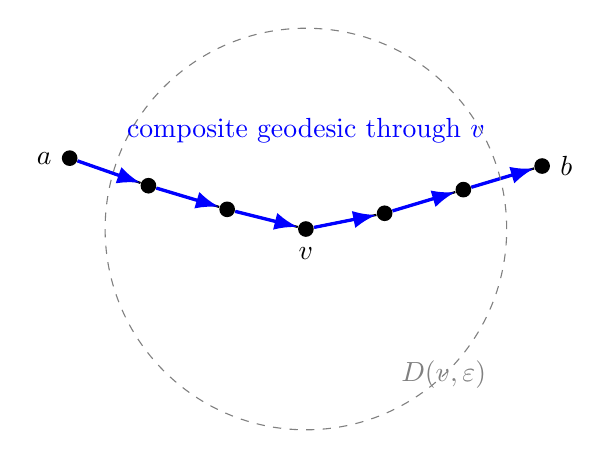
\begin{tikzpicture}[>=Latex,x=1cm,y=1cm]
  \node[circle,fill=black,inner sep=2pt,label=below:{\(v\)}] (v) at (0,0) {};
  \node[circle,fill=black,inner sep=2pt,label=left:{\(a\)}] (a) at (-3,0.9) {};
  \node[circle,fill=black,inner sep=2pt,label=right:{\(b\)}] (b) at (3,0.8) {};
  \node[circle,fill=black,inner sep=2pt] (l1) at (-2,0.55) {};
  \node[circle,fill=black,inner sep=2pt] (l2) at (-1,0.25) {};
  \node[circle,fill=black,inner sep=2pt] (r1) at (1,0.20) {};
  \node[circle,fill=black,inner sep=2pt] (r2) at (2,0.50) {};

  \draw[thick] (a) -- (l1) -- (l2) -- (v) -- (r1) -- (r2) -- (b);
  \draw[blue,very thick,->] (a) -- (l1);
  \draw[blue,very thick,->] (l1) -- (l2);
  \draw[blue,very thick,->] (l2) -- (v);
  \draw[blue,very thick,->] (v) -- (r1);
  \draw[blue,very thick,->] (r1) -- (r2);
  \draw[blue,very thick,->] (r2) -- (b);

  \draw[dashed,gray] (0,0) circle (2.55);
  \node[gray] at (1.75,-1.85) {\(D(v,\eps)\)};
  \node[blue] at (0,1.25) {composite geodesic through \(v\)};
\end{tikzpicture}
\caption{A composite geodesic path through \(v\) is built by joining two
shortest paths from \(v\) to disk-boundary vertices.  It is retained only when
the joined path is itself shortest between its endpoints.}
\end{figure}

\section{Pathwise Polynomial Annihilators}

Let
\[
  \gamma=(v_0,\ldots,v_m)\in \Geo(v,\eps)
\]
be a composite geodesic path containing \(v=v_j\).  Give this path a
one-dimensional coordinate system centered at \(v\):
\[
  t_j=0,
\]
\[
  t_i=-d_G(v_i,v)\quad \text{for } i<j,
  \qquad
  t_i=d_G(v_i,v)\quad \text{for } i>j.
\]

Now a function \(f:V\to\R\) restricted to \(\gamma\) becomes one-dimensional
data:
\[
  (t_i, f(v_i)),\qquad i=0,\ldots,m.
\]

\subsection{Exact Divided-Difference Rows}

If we use exactly \(r+2\) points along a path, then the \((r+1)\)-st divided
difference
\[
  [t_0,\ldots,t_{r+1}]f
\]
annihilates every degree-\(r\) polynomial in \(t\).  This gives a row vector
\[
  a_{\gamma}^{(r+1)}
\]
such that
\[
  a_{\gamma}^{(r+1)} f_\gamma = 0
\]
whenever \(f_\gamma\) is sampled from a polynomial of degree at most \(r\)
along the path.

\subsection{Regression-Based Rows}

For longer paths, it is often better to use all points on the path.  Let
\[
  X_\gamma =
  \begin{bmatrix}
  1 & t_0 & t_0^2 & \cdots & t_0^{r+1}\\
  1 & t_1 & t_1^2 & \cdots & t_1^{r+1}\\
  \vdots & \vdots & \vdots & & \vdots\\
  1 & t_m & t_m^2 & \cdots & t_m^{r+1}
  \end{bmatrix},
\]
and let \(W_\gamma\) be a diagonal kernel weight matrix centered at \(t=0\).
The weighted least-squares coefficient vector is
\[
  \widehat\alpha
  =
  (X_\gamma^T W_\gamma X_\gamma)^{-1}X_\gamma^TW_\gamma f_\gamma.
\]
The coefficient \(\widehat\alpha_{r+1}\) is a linear functional of the path
values:
\[
  \widehat\alpha_{r+1}
  =
  a_{\gamma}^{(r+1)} f_\gamma,
\]
where
\[
  a_{\gamma}^{(r+1)}
  =
  e_{r+2}^T
  (X_\gamma^T W_\gamma X_\gamma)^{-1}
  X_\gamma^T W_\gamma.
\]

This row also annihilates degree-\(r\) polynomials, because the fitted
\((r+1)\)-st coefficient is zero whenever the data lie exactly in the column
space of polynomials of degree at most \(r\).

\section{The Graph Operator}

For each vertex \(v\), each composite geodesic \(\gamma\in\Geo(v,\eps)\), and
degree \(r\), build a row \(a_{\gamma}^{(r+1)}\).  Assemble all rows into a
global sparse matrix:
\[
  A_{r+1,\mathrm{geo}}.
\]

The corresponding graph trend-filtering estimator is
\[
  \widehat f_\lambda
  =
  \argmin_{f\in\R^{|V|}}
  \left\{
  \frac12\norm{y-f}_2^2
  +
  \lambda\norm{A_{r+1,\mathrm{geo}}f}_1
  \right\}.
\]

The intended null-space property is
\[
  A_{r+1,\mathrm{geo}}f=0
  \quad\Longleftrightarrow\quad
  f \text{ is locally degree-\(r\) polynomial along sampled geodesics.}
\]

This is not automatically the same as a Euclidean multivariate polynomial
space.  It is a graph-intrinsic analogue.  On sufficiently rich samples of a
smooth manifold, however, this condition should approximate the smooth fact
that degree-\(r\) behavior along all lines through a point characterizes
degree-\(r\) polynomial behavior.

\section{Estimating Local Intrinsic Dimension}

The discussion above assumes that the local polynomial dimension is known.  On
a sampled square this is easy: the intrinsic dimension is two, so the dimension
of degree-\(r\) polynomials is
\[
  \dim \mathcal P_r(\R^2)
  =
  \binom{r+2}{2}.
\]
On a general graph, however, there is no given coordinate dimension.  A graph
disk may look one-dimensional near a boundary, two-dimensional in a sampled
surface region, or higher-dimensional near a highly branched or noisy part of
the graph.  Therefore a local row-selection rule should not require a fixed
dimension as a hidden assumption.

Let \(m_v\) denote the effective intrinsic dimension near vertex \(v\).  If
\(m_v\) were known, the local degree-\(r\) polynomial dimension would be
\[
  p_v(r)
  =
  \binom{m_v+r}{r}.
\]
For example,
\[
\begin{array}{c|ccc}
\toprule
m_v & r=1 & r=2 & r=3\\
\midrule
1 & 2 & 3 & 4\\
2 & 3 & 6 & 10\\
3 & 4 & 10 & 20\\
\bottomrule
\end{array}
\]
Thus the local dimension estimate directly determines the null-space size that
rank-based row thinning should try to preserve.

\subsection{Local MDS/PCA Dimension}

A simple geometric estimator starts from pairwise graph-geodesic distances
inside the disk \(D(v,\eps)\).  Apply classical multidimensional scaling
(MDS), or an equivalent local principal-coordinate analysis, to obtain
nonnegative local eigenvalues
\[
  \lambda_{v,1}\ge \lambda_{v,2}\ge \cdots \ge 0.
\]
The dimension can be estimated by an energy threshold:
\[
  \widehat m_v^{\mathrm{MDS}}
  =
  \min\left\{
  m:
  \frac{\sum_{j=1}^m \lambda_{v,j}}
       {\sum_{j\ge 1}\lambda_{v,j}}
  \ge \alpha
  \right\},
\]
with a default such as \(\alpha=0.90\) or \(0.95\).  An alternative is an
eigengap rule:
\[
  \widehat m_v^{\mathrm{gap}}
  =
  \argmax_j
  \frac{\lambda_{v,j}}{\lambda_{v,j+1}+\delta},
\]
where \(\delta>0\) prevents division by zero.

The advantage of the MDS/PCA view is that it gives both an estimated dimension
and a diagnostic spectrum.  If the local spectrum has a clear drop after two
components, then a two-dimensional polynomial target is well supported.  If the
spectrum decays slowly, then the graph disk does not provide a clean local
Euclidean model.

\subsection{Volume-Growth Dimension}

A more graph-native estimator uses the growth rate of balls.  For radii
\[
  0<\rho_1<\rho_2<\cdots<\rho_L\le \eps,
\]
compute
\[
  N_v(\rho_\ell)
  =
  |B_G(v,\rho_\ell)|.
\]
On an \(m\)-dimensional smooth space, one expects locally
\[
  N_v(\rho)\approx C_v \rho^m.
\]
Taking logs gives
\[
  \log N_v(\rho)
  \approx
  \log C_v + m\log \rho.
\]
Thus one can estimate
\[
  \widehat m_v^{\mathrm{growth}}
  =
  \text{slope of a local regression of }
  \log N_v(\rho)
  \text{ on }
  \log \rho.
\]
This estimator is intrinsic and does not require an embedding, but it is often
noisy on small graph disks because vertex counts are discrete and boundary
effects are strong.

\subsection{Doubling Dimension}

A related estimate compares ball counts at two radii:
\[
  \widehat m_v^{\mathrm{dbl}}(\rho)
  =
  \log_2
  \frac{|B_G(v,2\rho)|}{|B_G(v,\rho)|}.
\]
If the graph locally resembles an \(m\)-dimensional space, this ratio should be
near \(m\).  Doubling estimates are easy to compute and easy to interpret, but
they can be unstable when \(B_G(v,\rho)\) is very small or when \(2\rho\) is
already close to the disk boundary.

\subsection{Combining And Smoothing Dimension Estimates}

No single estimator should be trusted blindly.  A practical implementation can
compute several raw estimates:
\[
  \widehat m_v^{\mathrm{MDS}},\qquad
  \widehat m_v^{\mathrm{growth}},\qquad
  \widehat m_v^{\mathrm{dbl}}.
\]
These can be combined by a median, a trimmed mean, or a confidence-weighted
average:
\[
  \widehat m_v^{\mathrm{raw}}
  =
  \operatorname{Combine}
  \left(
  \widehat m_v^{\mathrm{MDS}},
  \widehat m_v^{\mathrm{growth}},
  \widehat m_v^{\mathrm{dbl}}
  \right).
\]
For example, the MDS estimate could receive high confidence when the eigengap
is large, while the growth estimate could receive low confidence when the
available radius range is narrow.

Because intrinsic dimension should usually vary slowly across a sampled
manifold-like graph, the raw estimates should then be smoothed over the graph.
One may use graph low-pass smoothing, local median smoothing, or kernel
regression over graph distance:
\[
  \widetilde m_v
  =
  \frac{
    \sum_{u\in B_G(v,h)}
    K\!\left(d_G(u,v)/h\right)
    \widehat m_u^{\mathrm{raw}}
  }{
    \sum_{u\in B_G(v,h)}
    K\!\left(d_G(u,v)/h\right)
  }.
\]
The final integer dimension can then be obtained by rounding or thresholding:
\[
  m_v^\star
  =
  \min\{m_{\max},\max\{1,\operatorname{round}(\widetilde m_v)\}\}.
\]

This smoothing step is important.  Without it, neighboring vertices may
alternate between dimensions \(1\), \(2\), and \(3\) because of small changes
in local sampling density.  Such flickering would make the row-selection rule
unstable.

\subsection{Use In Rank-Based Row Thinning}

Let
\[
  n_v=|D(v,\eps_v)|
\]
be the number of vertices in the local disk.  Once a smoothed dimension
estimate \(m_v^\star\) is available, the local polynomial dimension target is
\[
  p_v(r)
  =
  \binom{m_v^\star+r}{r}.
\]
If \(A_v^{\mathrm{cand}}\) is the matrix of all candidate annihilator rows for
the disk, then a rank-thinning rule can aim for local rank
\[
  \rank(A_v)
  \approx
  n_v-p_v(r).
\]
Equivalently, the local nullity target is
\[
  \dim\nullsp(A_v)
  \approx
  p_v(r).
\]

This suggests a constructive thinning algorithm:
\begin{enumerate}
  \item Generate candidate pathwise annihilator rows in \(D(v,\eps_v)\).
  \item Estimate \(m_v^\star\) from local graph geometry.
  \item Set the target local rank to \(n_v-\binom{m_v^\star+r}{r}\).
  \item Add candidate rows greedily only when they increase numerical rank or
        improve conditioning.
  \item Stop when the target rank is reached, or when all useful candidate
        rows have been exhausted.
\end{enumerate}

The dimension estimate should guide row thinning, not certify success.  The
operator still needs to be tested by numerical nullity and polynomial residuals:
\[
  \widehat{\dim\nullsp(A)}
  \quad\text{and}\quad
  \frac{\norm{A f_{\mathrm{poly}}}_2}{\norm{f_{\mathrm{poly}}}_2}.
\]
The purpose of estimating local dimension is to prevent row thinning from
silently imposing a two-dimensional polynomial target on graph regions whose
geometry is effectively one-dimensional, three-dimensional, branched, or too
irregular for a clean polynomial model.

\subsection{Using Local Nullity And Polynomial Residuals During Thinning}

The local dimension estimate is not the only information available during row
selection.  Once candidate rows have been generated on a disk, we can also
measure directly whether the selected rows preserve the intended polynomial
space.  The important distinction is local versus global use.

Let \(P_v\) be a local polynomial design matrix on \(D(v,\eps_v)\).  If local
coordinates \(z_u\in\R^{m_v^\star}\) have been estimated for vertices
\[
  u\in D(v,\eps_v),
\]
then \(P_v\) contains all monomials up to degree \(r\) in those local
coordinates.  For example, if \(m_v^\star=2\) and \(r=2\), then the columns are
\[
  1,\quad z_1,\quad z_2,\quad z_1^2,\quad z_1z_2,\quad z_2^2.
\]
For a candidate selected local row matrix \(A_{v,S}\), define the local
polynomial residual
\[
  \rho_v(S)
  =
  \frac{\norm{A_{v,S}P_v}_F}{\norm{P_v}_F}.
\]
Also define the local nullity estimate
\[
  \nu_v(S)=\dim\nullsp(A_{v,S}).
\]
The desired target is
\[
  \nu_v(S)\approx p_v(r)
  =
  \binom{m_v^\star+r}{r},
  \qquad
  \rho_v(S)\approx 0.
\]

Thus local nullity and local polynomial residuals can be used constructively
inside the thinning algorithm.  A useful row-selection objective is:
\[
  \min_{S\subseteq \mathcal R_v}
  \left\{
    \rho_v(S)
    +
    \mu\left|\nu_v(S)-p_v(r)\right|
    +
    \eta\,\kappa_v(S)
    +
    \zeta\,C_v(S)
  \right\},
\]
where \(\mathcal R_v\) is the candidate row set, \(\kappa_v(S)\) is a
conditioning penalty, and \(C_v(S)\) is a coverage penalty that discourages
selecting rows that ignore large parts of the disk or repeatedly use the same
paths.

A greedy version is often more practical:
\begin{enumerate}
  \item Start with no selected rows.
  \item Add a candidate row only if it increases numerical rank outside the
        current polynomial space.
  \item Reject rows that make \(\rho_v(S)\) too large.
  \item Stop when \(\nu_v(S)\) is close to \(p_v(r)\), or when no remaining row
        improves rank and coverage without damaging polynomial residuals.
\end{enumerate}

This is different from using the final global diagnostics as the proof that the
operator works.  If one chooses rows specifically to make a global test matrix
\(P_d\) satisfy
\[
  \frac{\norm{A P_d}_F}{\norm{P_d}_F}\approx 0,
\]
then the same quantity cannot be treated as independent evidence of success.
It becomes a construction criterion.  This is not wrong, but it must be
reported as such.

The clean experimental separation is:
\[
\begin{array}{ll}
\text{during construction:}
&
  \nu_v(S),\ \rho_v(S),\ \text{conditioning, and coverage on local disks},
\\[4pt]
\text{after construction:}
&
  \dim\nullsp(A),\
  \dfrac{\norm{A P_{\mathrm{test}}}_F}{\norm{P_{\mathrm{test}}}_F},\
  \text{and held-out synthetic graph tests}.
\end{array}
\]
In other words, local nullity and local polynomial residuals should guide
thinning.  Global nullity and global residuals should remain final diagnostics,
preferably evaluated on polynomial probes or synthetic examples not used to
select the rows.

\section{Example: Path Graph}

Consider the path graph
\[
  1-2-\cdots-n.
\]
For an interior vertex \(v=i\), a graph disk produces a left ray and a right
ray.  The composite geodesic through \(i\) is simply an interval of the path:
\[
  i-q,\ldots,i,\ldots,i+q.
\]

For \(r=2\), the annihilator is third order.  On equally spaced vertices, a
four-point window gives the familiar row
\[
  [-1,\ 3,\ -3,\ 1].
\]
Therefore the geodesic construction reduces to ordinary one-dimensional
quadratic trend filtering on path graphs, up to the boundary and window
selection convention.

\begin{figure}[ht]
\centering
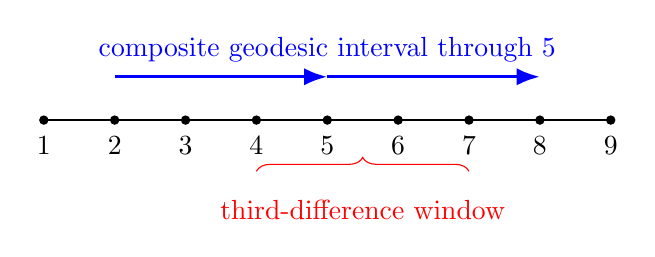
\begin{tikzpicture}[x=0.9cm,y=1cm,>=Latex]
  \foreach \i in {1,...,9} {
    \fill[black] (\i,0) circle (1.7pt);
    \node[below] at (\i,-0.08) {\(\i\)};
  }
  \draw[thick] (1,0) -- (9,0);
  \draw[blue,very thick,->] (2,0.55) -- (5,0.55);
  \draw[blue,very thick,->] (5,0.55) -- (8,0.55);
  \node[blue,above] at (5,0.62) {composite geodesic interval through \(5\)};
  \draw[red,decorate,decoration={brace,amplitude=5pt}] (4,-0.65) -- (7,-0.65);
  \node[red,below=7pt] at (5.5,-0.65) {third-difference window};
\end{tikzpicture}
\caption{On a path graph, composite geodesics are ordinary intervals.  The
\((r+1)\)-st pathwise annihilator recovers the usual one-dimensional
trend-filtering difference rows.}
\end{figure}

\section{Example: Three-Arm Star}

Now consider a three-arm star with two vertices per arm:
\[
  u-v_{a1}-v_{a2},
  \qquad a=1,2,3.
\]
Composite geodesics through the center \(u\) include cross-arm paths such as
\[
  v_{11}-u-v_{21}.
\]

For \(r=1\), the annihilator is second order.  With equal edge lengths, the
cross-arm row is
\[
  f_{11}-2f_u+f_{21}.
\]
If every cross-arm second difference vanishes, then the slopes across arms are
forced to be compatible.  With only one vertex per arm, the null space can
collapse to constants.  With longer arms, the condition says something closer
to: values should extend linearly through the branch point along every
geodesic line that passes through it.

\begin{figure}[ht]
\centering
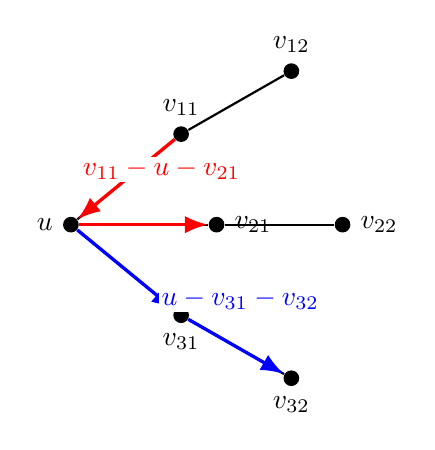
\begin{tikzpicture}[>=Latex,x=1cm,y=1cm]
  \node[circle,fill=black,inner sep=2pt,label=left:{\(u\)}] (u) at (0,0) {};
  \node[circle,fill=black,inner sep=2pt,label=above:{\(v_{11}\)}] (v11) at (1.4,1.15) {};
  \node[circle,fill=black,inner sep=2pt,label=above:{\(v_{12}\)}] (v12) at (2.8,1.95) {};
  \node[circle,fill=black,inner sep=2pt,label=right:{\(v_{21}\)}] (v21) at (1.85,0) {};
  \node[circle,fill=black,inner sep=2pt,label=right:{\(v_{22}\)}] (v22) at (3.45,0) {};
  \node[circle,fill=black,inner sep=2pt,label=below:{\(v_{31}\)}] (v31) at (1.4,-1.15) {};
  \node[circle,fill=black,inner sep=2pt,label=below:{\(v_{32}\)}] (v32) at (2.8,-1.95) {};
  \draw[thick] (u) -- (v11) -- (v12);
  \draw[thick] (u) -- (v21) -- (v22);
  \draw[thick] (u) -- (v31) -- (v32);
  \draw[red,very thick,->] (v11) -- (u);
  \draw[red,very thick,->] (u) -- (v21);
  \node[red,fill=white,inner sep=1pt] at (1.15,0.70) {\(v_{11}-u-v_{21}\)};
  \draw[blue,very thick,->] (u) -- (v31);
  \draw[blue,very thick,->] (v31) -- (v32);
  \node[blue,fill=white,inner sep=1pt] at (2.15,-0.95) {\(u-v_{31}-v_{32}\)};
\end{tikzpicture}
\caption{A star graph exposes a modeling choice.  Composite geodesics include
cross-arm paths through the center; arm-continuation paths are only a subset.
Cross-arm rows enforce compatibility of polynomial behavior across arms.}
\end{figure}

This is not a flaw.  It is a choice.  The composite-geodesic construction treats
two arms that form a shortest path through \(u\) as two sides of a local
geodesic line.  If the scientific goal is branch-specific slopes, use fewer
paths.  If the goal is a graph analogue of line tests through a point, keep the
composite geodesics.

\section{What Should Happen on Sampled Squares?}

The computational test that matters most is a graph built from points sampled
from
\[
  [0,1]^2.
\]
Construct a symmetric \(k\)-nearest-neighbor graph, with edge lengths inherited
from Euclidean distances.  Around each vertex, choose a disk radius \(\eps\)
and build composite geodesics.

For degree \(r=1\), the null space should approximately contain affine
functions:
\[
  f(x,y)=a+bx+cy.
\]
For degree \(r=2\), it should approximately contain quadratics:
\[
  f(x,y)=a+bx+cy+d x^2+e xy+g y^2.
\]
For degree \(r=3\), it should approximately contain cubics:
\[
\begin{split}
  f(x,y)=&\,a+bx+cy+d x^2+e xy+g y^2\\
         &+h x^3+i x^2y+j xy^2+k y^3.
\end{split}
\]

The dimensions in two variables are
\[
  \dim \mathcal P_r(\R^2)=\binom{r+2}{2}.
\]
Thus the expected dimensions are:
\[
\begin{array}{c|c|c}
\toprule
r & \text{polynomial space} & \dim \mathcal P_r(\R^2)\\
\midrule
1 & \text{affine} & 3\\
2 & \text{quadratic} & 6\\
3 & \text{cubic} & 10\\
\bottomrule
\end{array}
\]

On a finite noisy graph, the nullity of \(A_{r+1,\mathrm{geo}}\) may not be
exactly these numbers.  A more stable diagnostic is:
\[
  \frac{\norm{A_{r+1,\mathrm{geo}}f_{\mathrm{poly}}}_2}
       {\norm{f_{\mathrm{poly}}}_2}
  \approx 0
\]
for sampled polynomial signals \(f_{\mathrm{poly}}\).

\section{What Should Happen on Sampled Quadrics?}

A second useful test is to sample a curved surface, for example
\[
  (x,y,z)=(x,y,x^2+y^2),
  \qquad (x,y)\in[0,1]^2,
\]
or more generally
\[
  z=q(x,y).
\]
Build the graph using Euclidean distances in \(\R^3\), or intrinsic graph
distances approximating the surface metric.

The expected behavior changes subtly.  A function that is quadratic in the
ambient coordinates \((x,y,z)\) is not the same as a quadratic in intrinsic
surface coordinates.  For example, the coordinate function
\[
  z=x^2+y^2
\]
is quadratic in the parameter coordinates \((x,y)\), but it is linear in the
ambient coordinate \(z\).

Therefore quadrics test two questions:

\begin{enumerate}
  \item Does the graph operator annihilate polynomials in intrinsic local
        geodesic coordinates?
  \item Does it behave differently from an operator built from ambient
        Euclidean coordinates?
\end{enumerate}

This is useful because the graph construction should be metric-intrinsic.  It
should depend primarily on graph geodesic geometry, not on the arbitrary
ambient coordinates used to store the samples.

\section{Suggested Computational Diagnostics}

For each graph and degree \(r=1,2,3\), build \(A_{r+1,\mathrm{geo}}\) and run
the following checks.

\subsection{Polynomial Residual Tests}

Sample known polynomial signals and compute:
\[
  \rho(f)
  =
  \frac{\norm{A_{r+1,\mathrm{geo}}f}_2}
       {\norm{f}_2}.
\]
For a good degree-\(r\) graph polynomial annihilator, \(\rho(f)\) should be
small for degree-\(r\) polynomial signals and larger for degree-\((r+1)\)
signals.

\subsection{Numerical Nullity}

Compute the singular values of \(A_{r+1,\mathrm{geo}}\).  Estimate nullity by
counting singular values below a tolerance:
\[
  \widehat{\dim\nullsp(A)}
  =
  \#\{s_i(A): s_i(A) < \tau\}.
\]
On sampled \([0,1]^2\), compare this with
\[
  \binom{r+2}{2}.
\]

\subsection{Local Nullity}

Because the operator is built from graph disks, global nullity can be distorted
by boundaries, irregular sampling, or disconnected path families.  Also compute
local nullity on each disk:
\[
  A_{r+1,\mathrm{geo}}|_{D(v,\eps)}.
\]
This reveals whether each local graph disk has the right polynomial degrees of
freedom.

\subsection{Boundary Diagnostics}

At boundary vertices, there may be too few balanced geodesics.  The graph path
Laplacian manuscript proposes mirror extensions for this problem.  The same
idea can be reused here: when only one geodesic ray is available, mirror the
ray to create a symmetric path and construct the annihilator on the mirrored
coordinate system.

\section{Implementation Sketch}

The construction can be organized as follows.

\begin{enumerate}
  \item For each vertex \(v\), compute \(D(v,\eps)\) and its boundary.
  \item Enumerate boundary pairs \((a,b)\).
  \item Keep composite paths \(a\to v\to b\) that are geodesic between \(a\)
        and \(b\).
  \item Assign signed path coordinates centered at \(v\).
  \item Build a divided-difference or weighted-regression annihilator row for
        degree \(r\).
  \item Insert the row into the global sparse matrix
        \(A_{r+1,\mathrm{geo}}\).
  \item Return diagnostics: number of disks, number of paths, boundary/mirror
        counts, row rank, estimated nullity, and polynomial residual tests.
\end{enumerate}

\section{Implementation Roadmap}

The mathematical construction above is intentionally broader than the first
computational implementation should be.  The near-term implementation should
therefore proceed as a sequence of auditable pieces: first build graph disks
and candidate geodesic-path rows, then add local coordinate and dimension
diagnostics, then use these diagnostics to thin rows and test the resulting
operator.

\subsection{Local Disk Construction}

For each vertex \(v\), construct a graph disk
\[
  D(v,\eps_v)=\{u:\dist_G(u,v)\leq \eps_v\}.
\]
The radius should be allowed to adapt by vertex.  A useful first rule is:
choose the smallest radius \(\eps_v\) for which the number of usable composite
geodesics through \(v\) reaches a requested minimum, subject to a maximum
radius and a maximum number of retained paths.  The implementation should
record the selected radius, disk size, number of candidate composite geodesics,
number of retained geodesics, and whether the maximum radius or path cap was
hit.

This adaptive-radius rule is important because fixed-radius disks can be too
sparse near boundaries or in locally irregular regions, while overly large
disks can mix distinct geometric regimes.

\subsection{Local Coordinate Engines}

Local coordinates are not part of the definition of the pathwise annihilator,
but they are useful for diagnostics, dimension estimation, and polynomial
probe construction.  The first implementation should support at least two
local embedding backends:
\[
  \texttt{cmdscale}
  \quad\text{and}\quad
  \texttt{weighted\_grip\_edge\_kk}.
\]
The \(\texttt{cmdscale}\) backend gives a classical metric-MDS reference from
local graph-geodesic distances.  The weighted-GRIP \(\to\) edge-KK backend
should use the weighted GRIP initializer followed by edge-restricted
Kamada--Kawai repair:
\[
  \texttt{grip.layout.weighted()}
  \;\longrightarrow\;
  \texttt{grip.optimize.edge.kk.layout()}.
\]
This is attractive because it attempts to realize the observed weighted graph
edge lengths directly, rather than only matching all-pairs distances through a
dense MDS objective.

The current weighted-GRIP \(\to\) edge-KK workflow is most mature for target
dimensions \(1,2,3\).  When the best three-dimensional local layout still has
large edge stress, the implementation should set a diagnostic flag rather than
silently treating the disk as intrinsically three-dimensional.

\subsection{Local Dimension Estimation}

The local intrinsic dimension estimate \(m_v\) should be treated as an
engineering guide, not as a proof of the operator's null space.  Candidate
dimension estimates can be obtained from several sources:

\begin{enumerate}
  \item edge-stress elbows from local weighted-GRIP \(\to\) edge-KK embeddings
        in dimensions \(1,2,3\);
  \item singular-value or eigenvalue elbows from local coordinates;
  \item spectral diagnostics of the local graph Laplacian or local heat
        kernel;
  \item smoothed estimates obtained by regressing raw vertexwise estimates
        over the graph.
\end{enumerate}

The implementation should keep the individual diagnostic votes as well as the
selected dimension.  In particular, a local dimension cap should be visible in
the output when the evidence suggests dimension greater than three.

\subsection{Candidate Path Rows}

For each disk \(D(v,\eps_v)\), generate candidate composite geodesic paths and
convert them into \((r+1)\)-st pathwise divided-difference rows.  The first
implementation should include:

\begin{enumerate}
  \item a cap on the number of candidate composite geodesics per vertex;
  \item random tie-breaking when multiple shortest paths exist between the
        same boundary pair;
  \item mirror extensions at graph boundaries and in sparse one-sided local
        neighborhoods;
  \item row-level diagnostics recording path length, endpoint distance, disk
        radius, and whether the row used a mirror extension.
\end{enumerate}

The row-normalization rule should remain configurable because it changes the
effective penalty.  Important variants include no normalization, path-length
normalization, disk/path-count normalization, and vertex-level normalization.

\subsection{Row Thinning}

Candidate rows can easily overconstrain dense or high-degree graph disks.  Row
thinning should therefore be a first-class part of the implementation rather
than a post-hoc clean-up step.  A useful local objective is to choose rows that
keep a local polynomial design \(P_v\) nearly unpenalized while still providing
coverage and rank outside that polynomial space:
\[
  \frac{\norm{A_vP_v}_F}{\norm{P_v}_F}
  \approx 0.
\]
At the same time, selected rows should improve path coverage, avoid extreme
conditioning, and move local nullity toward the dimension of the desired
polynomial probe space.

This means that local dimension estimates guide the thinning target, while the
actual thinning criterion uses the rows themselves:
\[
  \dim\nullsp(A_v),
  \qquad
  \frac{\norm{A_vP_v}_F}{\norm{P_v}_F},
  \qquad
  \text{coverage}(A_v).
\]

\subsection{Global Validation}

After local rows are assembled into the global operator, the final check should
be empirical.  The main validation quantities are:
\[
  \widehat{\dim\nullsp(A)},
  \qquad
  \frac{\norm{AP_d}_F}{\norm{P_d}_F},
\]
where \(P_d\) contains held-out polynomial probe signals of the target degree.
For sampled two-dimensional domains, the expected polynomial dimensions are
\[
  3,\quad 6,\quad 10
\]
for degrees \(1,2,3\), respectively.  These numbers should be treated as
reference targets for well-sampled planar examples, not as universal graph
truths.

\subsection{Experimental Graph Families}

The first validation suite should include graphs that isolate different
failure modes:

\begin{enumerate}
  \item path graphs, where the operator should reduce to ordinary
        one-dimensional divided differences;
  \item star and multi-arm graphs, where branching behavior and null-space
        inflation are easiest to inspect;
  \item sampled \([0,1]^2\) graphs, where degree-\(1,2,3\) polynomial nullities
        can be compared with \(3,6,10\);
  \item sampled quadrics over \([0,1]^2\), which test whether the operator is
        intrinsic rather than an ambient-coordinate annihilator;
  \item Delaunay one-skeleton graphs;
  \item symmetric kNN and continuous-kNN graphs.
\end{enumerate}

For each family, reports should show disk-size histograms, composite-geodesic
histograms, selected-radius diagnostics, local dimension diagnostics,
polynomial residuals, and numerical nullity.

\section{Interpretation}

The graph path Laplacian manuscript used composite geodesics to estimate an
average of second directional derivatives.  The present construction uses the
same geodesic sampling idea, but changes the target:

\[
\text{path Laplacian: estimate and average second derivatives,}
\]
\[
\text{polynomial annihilator: penalize \((r+1)\)-st pathwise derivatives.}
\]

For \(r=2\), this means penalizing third pathwise derivatives.  The intended
effect is the graph analogue of quadratic trend filtering: functions that are
locally quadratic along sampled geodesic lines should be nearly unpenalized,
while deviations from local quadratic behavior should be sparse and adaptive.

\section{Open Questions}

\begin{enumerate}
  \item Should \(\Geo(v,\eps)\) include all composite geodesics, or a sampled
        subset for computational stability?
  \item How should multiple shortest paths between the same boundary pair be
        handled?
  \item Should path rows be normalized by path length, disk size, or number of
        paths through \(v\)?
  \item Should mirror extensions be used only at graph boundaries, or also in
        sparse one-sided local neighborhoods?
  \item On sampled \([0,1]^2\), does the estimated nullity stabilize near
        \(3,6,10\) for degrees \(1,2,3\)?
  \item On sampled quadrics, does the operator behave like an intrinsic
        polynomial annihilator rather than an ambient coordinate polynomial
        annihilator?
\end{enumerate}

\section{Summary}

The proposed operator is a graph-intrinsic polynomial annihilator:
\[
  A_{r+1,\mathrm{geo}}f
\]
is built by sampling composite geodesic paths through graph disks and applying
\((r+1)\)-st one-dimensional polynomial annihilators along those paths.  It
inherits the motivating idea of the graph path Laplacian, but targets graph
trend filtering rather than quadratic spectral smoothing.  On path graphs it
reduces to ordinary one-dimensional trend-filtering differences.  On richer
graphs it gives a way to test whether local graph signals behave like
degree-\(r\) polynomials along intrinsic geodesic directions.

\end{document}
